\documentclass[10pt]{scrartcl}
\usepackage{graphicx}
\usepackage{float}
\usepackage{amsmath}
\usepackage[utf8]{inputenc} 
\usepackage[T1]{fontenc}
\usepackage{lmodern}
\usepackage{amsfonts}   
\usepackage{amssymb}
\usepackage{mathtools}

 
\begin{document}
\title{Praktiukumsarbeit zum Praktikum Regelungstechnik}
\author{Christian Küllmer, Jonas Kallweidt, Leon Blum}
\date{\today{}, Kassel}
\maketitle
\newpage
%Inhaltsverzeichnis
\renewcommand{\contentsname}{Inhaltsverzeichnis}
\tableofcontents
\newpage

%Mathlab Aufgabe
\section{Rechnerteil Aufgaben aus Kapitel 9.3. des Praktikumsskrips}
In diesem Anteil geht es um die in Aufgabe 9.3a. Dieser bezeichnet das Aufstellen der Gleichungen aus den gegeben Gleichungen. Die Gleichungen sind gegen als Blockschaltbild gegeben. Diese werden jetzt übersetzt in Mathlab Simulink.

%\begin{itemize}
%\item Startwerte
%Als Startwerte wurde gegeben:

%\begin{align}
%   	c &= 1 \\k &= 300  \\ T& = 0,1\\ g &= 9,81\, \frac{m}{s^2} \\l &= 1\, m\\m &= 7\, kg
%\end{align}

	
	


%\item Gegebenes Blockschaltbild:
%\begin{figure}[H]
%	\centering
%	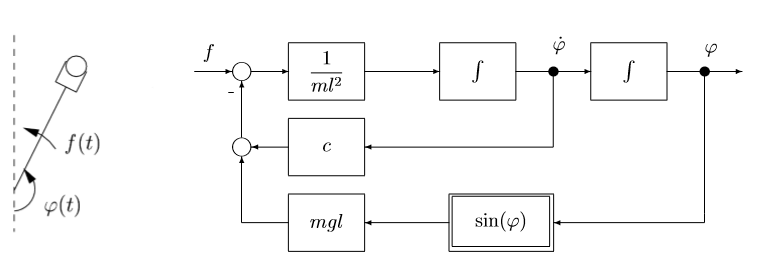
\includegraphics[width=0.6\textwidth]{Aufgabe9aMotorarm.png}
%	\caption{Motorarmmodell als Blockschaltbild}
%	\label{img:grafik-dummy}
%\end{figure}
%\begin{figure}[H]
%	\centering
%	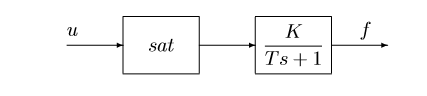
\includegraphics[width=0.6\textwidth]{Aufgabe9aStreckeMotor.png}
%	\caption{Modell des Motors als Blockschaltbild}
%	\label{img:grafik-dummy}
%\end{figure}
%\end{itemize}

\subsection{Wichtiger Hinweis:}
Für alle in diesem Bereich folgenden Auswertungen gibt folgende Farbkonvention
\begin{itemize}
\item Die rote Kurve entspricht dem Winkel $\varphi$
\item Die blaue Kurve entspricht dann der Winkelgeschwindigkeit $\dot \varphi$
\item Die grüne Kurve entspricht der Winkelbeschleunigung  $ \ddot \varphi$
\end{itemize}

%Version von Jonas und Christian vom 24.07.2019

\subsection{Aufgabe a) Gebautes Simulink Modell}
\begin{figure}[H]
	\centering
	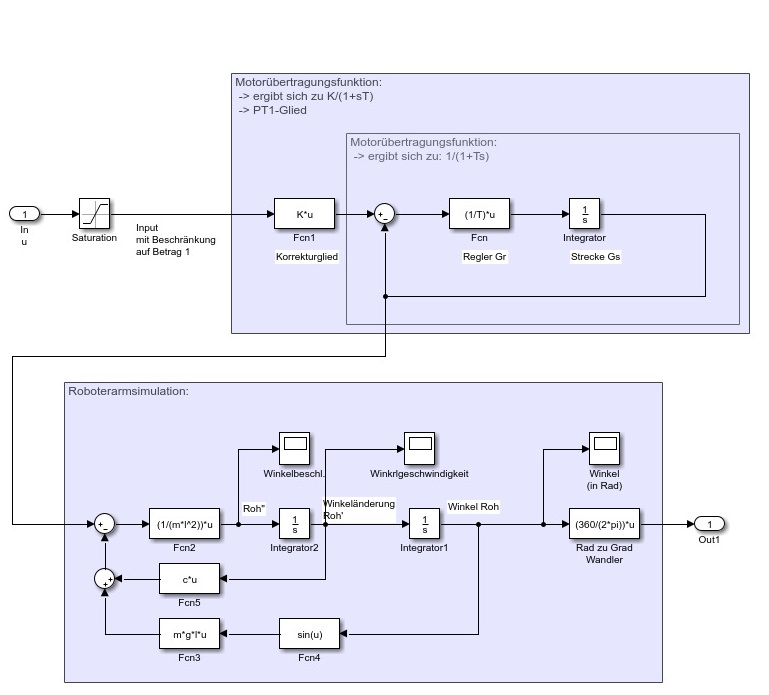
\includegraphics[width=0.7\textwidth]{SimulinkModell.jpeg}
	\caption{In Simulink gebautes Modell des Systems des Roboterarms}
	\label{img:grafik-dummy}
\end{figure}

%Version von Jonas und Christian vom 24.07.2019
\newpage
\subsection{Aufgabe b)}
Das System wird simuliert und die Zustandsgrößen werden über einen Zeitverlauf dargestellt. Dabei entstehen folgende Diagramme:

\begin{figure}[H]
	\centering
	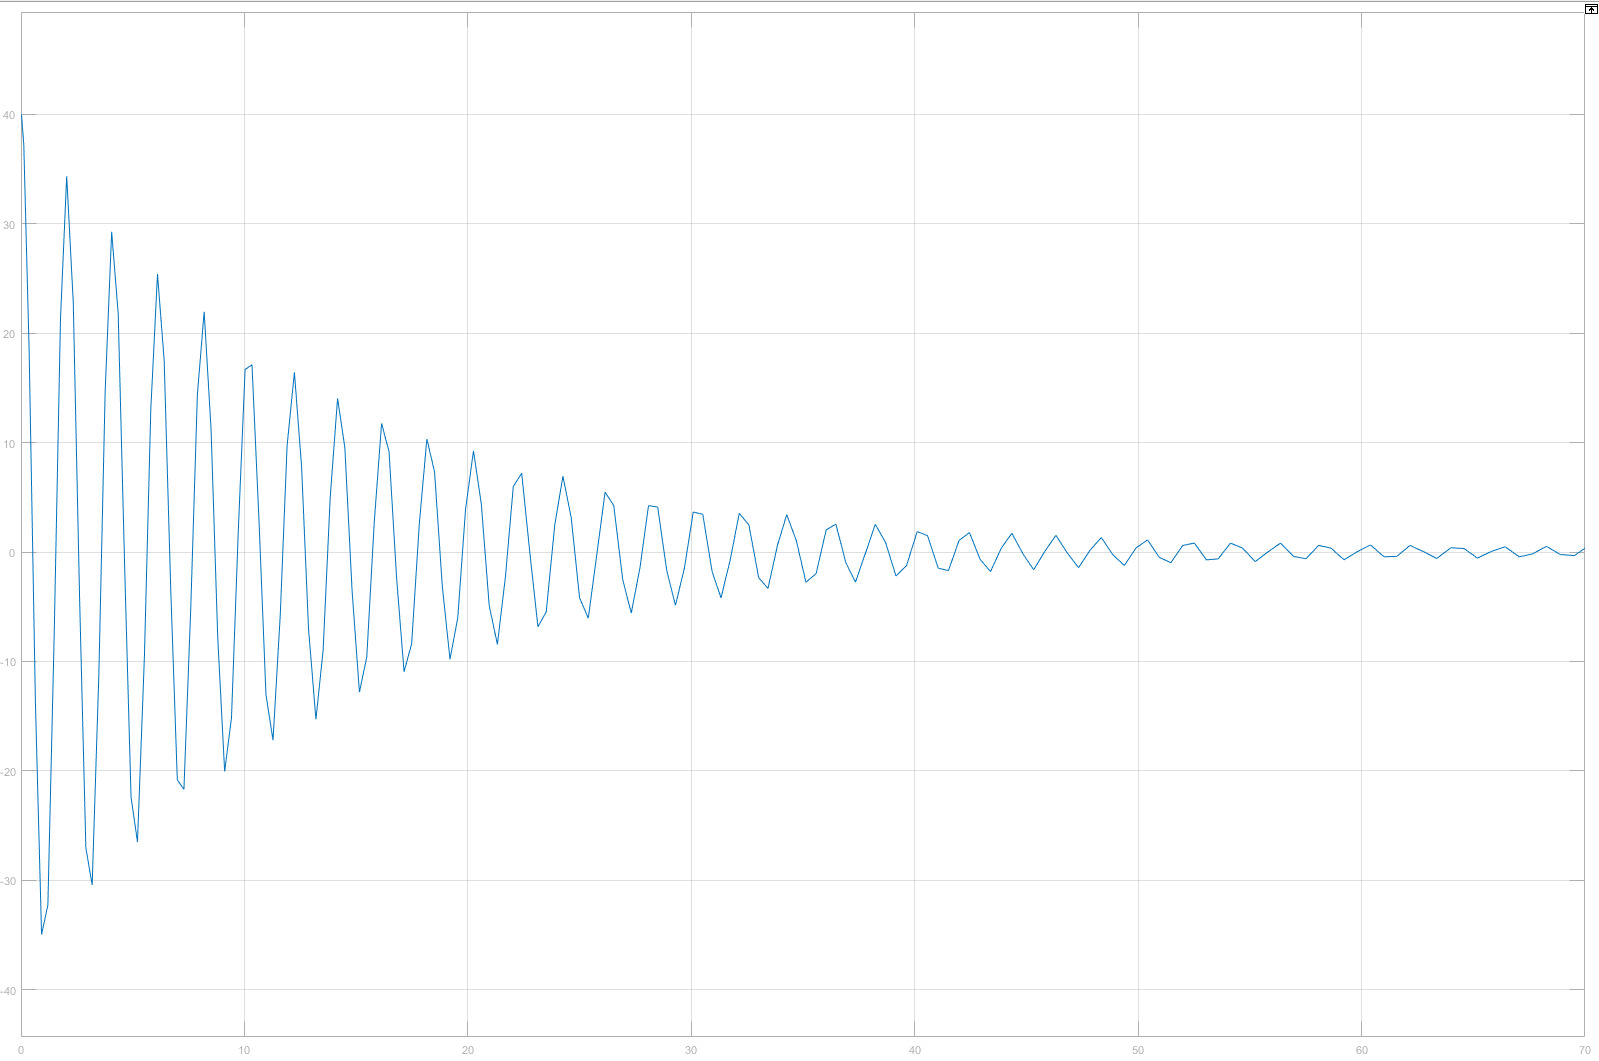
\includegraphics[width=1\textwidth]{WinkelanzeigeinGrad3b.jpeg}
	\caption{Darstellung des Winkels für eine anfängliche Auslenkung von 40 Grad. }
	\label{img:grafik-dummy}
\end{figure}
Aus dem Diagramm Figure 4 geht hervor, dass das System ein ungeregelt stabiles System darstellt, welches eine Ruhelage bei 0\,$^\circ$ annehmen kann, wenn vorher keine Auslenkung vorgenommen wurde. Hier geht die Auslenkung auf keinen stationären Endwert, da die Expotentialfunktion zur Beschreibung der Dämpfung niemals null wird. In einem Realen System wird hier aber wahrscheinlich ein Stillstand nach beliebig langer Wartezeit eintreten, wenn der Roboterarm die Haftreibung nicht mehr Überwinden kann und die Bewegung im Aperiodischen Grenzfall endet.

%Version von Jonas und Christian vom 24.07.2019
\newpage
\subsection{Aufgabe c)}
Es soll eine Simulation angezeigt werden, die die Startwerte 

\begin{align}
\varphi  (0) &= 0 \\
\dot \varphi (0) &= 0 \\
u(t)  &= \binom{0\,\,\,\,\,\,\,\,\, für\,\, t<1}{0.17\,\, für\,\, t \geq 1}
\end{align}
\begin{figure}[H]
	\centering
	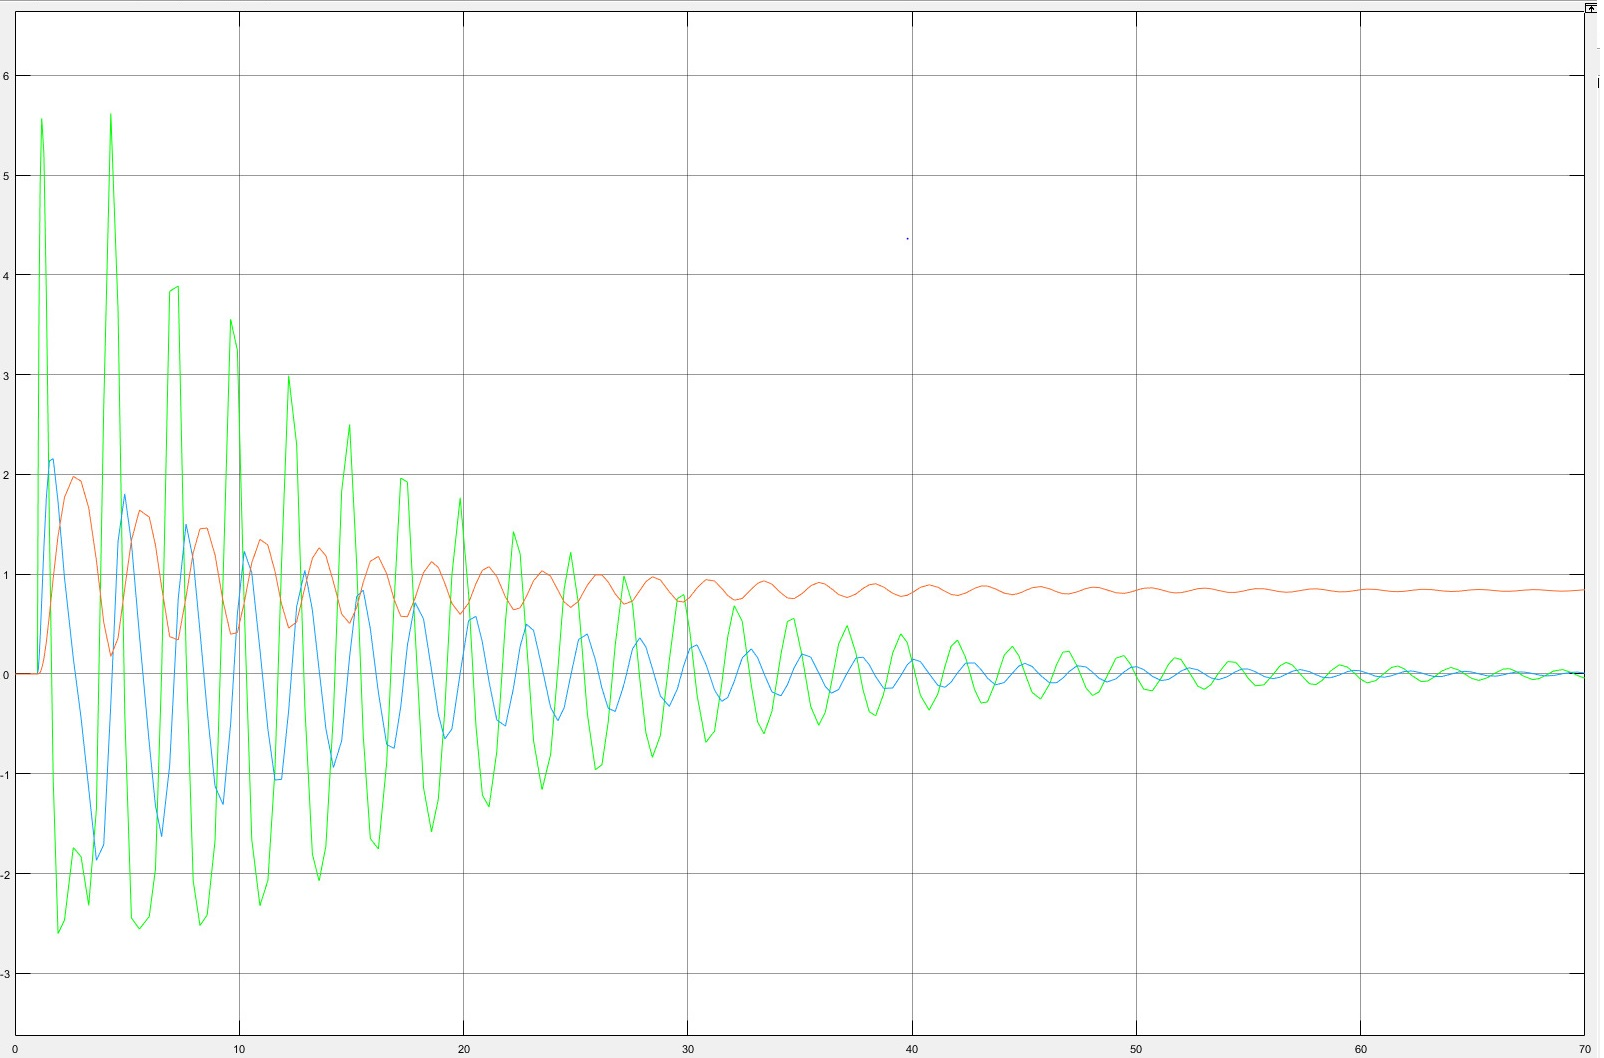
\includegraphics[width=0.8\textwidth]{Aufgabe9c.jpeg}
	\caption{Darstellung des Winkels für eine anfängliche Auslenkung von 40 Grad. }
	\label{img:grafik-dummy}
\end{figure}
Das System befindet sich zunächst in Ruhelage
zum Zeitpunkt t=1 wird ein Drehmoment vom Motor aufgebaut,
das den Roboterarm nach Durchlaufen eines Einschwingvorgangs 
um die neue Ruhelage in eben diese auslenkt . Diese neue Ruhelage hängt von dem Eingangsdrehmoment ab. Der Einschwingvorgang hat dabei ein gleiches Verhalten, wie der Einschwingvorgang von Aufgabe 9.3.b). 


%\varphi (0) &= 0 
%f(0) &= 0 
%
%u(t) &= 0 für t<1\\
%	0.17 für t >= 1;





%Das Simulinkmodell des Roboterarms wird für die entsprechende Schaltung verändert. Alle Veränderungen werden in dieser Grafik dokumentiert.
%Danach wird das Modell linearisiert und das dann entstehende Ergebnis wird

\subsection{Aufgabe d}
\begin{align}
\varphi  (0) &= 0 \\
\dot \varphi (0) &= 0 \\
u(t)  &= \binom{0\,\,\,\,\,\,\,\,\, für\,\, t<1}{0.18\,\, für\,\, t \geq 1}
\end{align}
\begin{figure}[H]
	\centering
	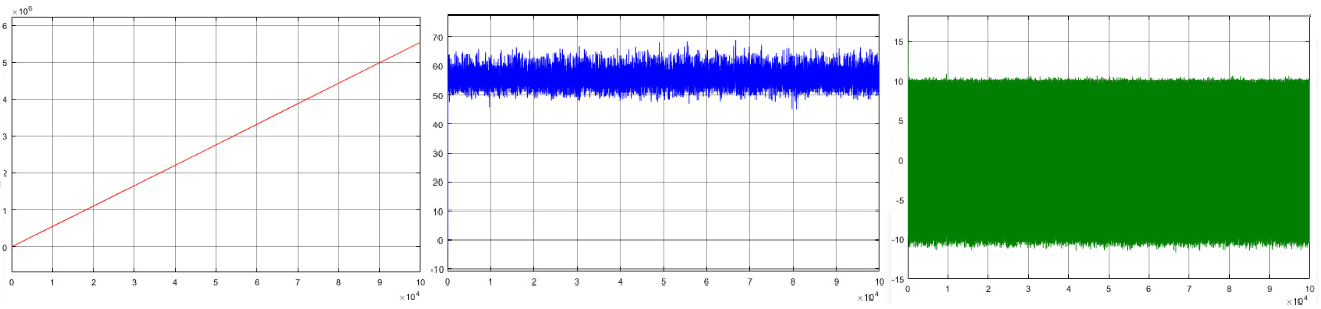
\includegraphics[width=1.2\textwidth]{Aufgabe9c.png}
	\caption{Darstellung des Winkels für eine anfängliche Auslenkung von 40 Grad. }
	\label{img:grafik-dummy}
\end{figure}

zu 3d:
Anders als im Versuch 9.3c befindet sich der Roboterarm nun zum Zeitpunkt
t = 0 nicht mehr in der Ruhelage bei einem Winkel von 0\,$^\circ$, sondern in einem 
Winkel von 40\,$^\circ$. Dies hat zur Folge, dass der Arm zunächst 
in der Zeit bis t = 1*s
sowie in der darauffolgenden Sättigungszeit des pt1 Gliedes,
das den Motor beschreibt, zurückschwingen kann.
Sobald das Drehmoment des Motors aufgebaut ist legt der Roboterarm 
an Geschwindigkeit zu und überschreitet dabei sogar die kritische 180\,$^\circ$
Marke, ab der der Arm nicht mehr zurückschwingt, sondern einen Überschlag
vollführt und weiter an Geschwindigkeit gewinnt.
Da es sich bei dem betrachtetet Roboterarm um ein gedämpftes Model
handelt, geht die Gewschwindigkeit in eine Sättigung über, bis diese um
einen konstanten Wert fluktuiert.
 %$ \alpha\beta\gamma\delta\epsilon\varepsilon\zeta\eta\theta\vartheta\iota\kappa\lambda\mu\nu\xi\pi
 %\varpi\rho\varrho\sigma\varsigma\tau\upsilon\phi\varphi\chi\psi\omega\Gamma\Delta\Theta\Lambda\Xi
 %\Pi\Sigma\Upsilon\Phi\Psi\Omega $



%Präsensversuche
\section{Versuch Antrieb}

\section{Versuch Schwebekörper}

\section{Versuch Kran}

%Modell zum Einfügen eines Bildes
%\begin{figure}[H]
%	\centering
%	\includegraphics[width=0.8\textwidth]{}
%	\caption{Teamlogo: Team A}
%	\label{img:grafik-dummy}
%\end{figure}
Hallo
\begin{figure}[H]
	\centering
	\includegraphics[width=1.2\textwidth]{untitled1.fig}
	\caption{Darstellung des Winkels für eine anfängliche Auslenkung von 40 Grad. }
	\label{img:grafik-dummy}
\end{figure}

\end{document}